\documentclass{beamer}
\usetheme{Warsaw}

\usepackage{enumerate}
\usepackage{soul}
\usepackage{xcolor}
\usepackage{hyperref}

\setbeamertemplate{footline}
{
  \leavevmode
  \hbox{
    \begin{beamercolorbox}[wd=.4\paperwidth,ht=2.25ex,dp=1ex,center]{author in head/foot}
        \usebeamerfont{whitespace}
    \end{beamercolorbox}
    \begin{beamercolorbox}[wd=.2\paperwidth,ht=2.25ex,dp=1ex,center]{title in head/foot}
        \hspace*{1em}
        \insertframenumber{}
        \hspace*{1em}
    \end{beamercolorbox}
    \begin{beamercolorbox}[wd=.4\paperwidth,ht=2.25ex,dp=1ex,center]{author in head/foot}
        \usebeamerfont{whitespace}
    \end{beamercolorbox}
  }
}

\makeatletter
\setbeamertemplate{navigation symbols}{}

\title[Or how my wife started forgetting about my ability to wreck a home network]{Nix}
\subtitle{Newcastle Cybersecurity Group}
\author[Jay Rovacsek]{Jay Rovacsek}
\date{\today}

\begin{document}

\begin{frame}
    \maketitle
\end{frame}

\section{Introduction}
\subsection{\$whoami}

\begin{frame}
    \begin{center}
        Public speaking skills: a solid 2.75/10 - remind me now that I should slow down and chill-out
    \end{center}
\end{frame}

\begin{frame}
    \begin{center}
        Wait a minute - you used that slide last year.
    \end{center}
\end{frame}

\begin{frame}
    \begin{center}
        Yep! This talk is somewhat of a follow-on of the Feb 2021 session
    \end{center}
\end{frame}

\begin{frame}
    \begin{columns}
        \begin{column}{0.5\textwidth}
            If you have questions at any point feel free to jump in!
        \end{column}
        \begin{column}{0.5\textwidth}
            \begin{figure}
                \centering
                
\includegraphics[width=\textwidth,keepaspectratio]{../resources/question.png}
            \end{figure}
        \end{column}
    \end{columns}
\end{frame}

\begin{frame}
    \begin{columns}
        \begin{column}{0.5\textwidth}
            \$whoami: I do cybers, but also very keen on:
            \begin{itemize}
                \item Chasing my kids around
                \item Generation 1 Pokemon, as others are inferior
                \item Picking up heavy things and putting them down
            \end{itemize}
        \end{column}
        \begin{column}{0.5\textwidth}
            \begin{figure}
                \centering
                
\includegraphics[width=\textwidth,keepaspectratio]{../resources/smile.jpg}
            \end{figure}
        \end{column}
    \end{columns}
\end{frame}

\begin{frame}
    \begin{columns}
        \begin{column}{0.5\textwidth}
            What am I still not?
            \begin{itemize}
                \item A sysadmin
                \item Good at making presentation slides
            \end{itemize}
        \end{column}
        \begin{column}{0.5\textwidth}
            \begin{figure}
                \centering
                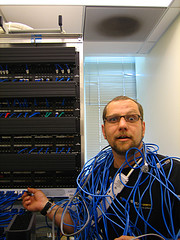
\includegraphics[width=\textwidth,keepaspectratio]{../resources/sysadmin.jpg}
            \end{figure}
        \end{column}
    \end{columns}
\end{frame}

\begin{frame}
    \begin{columns}
        \begin{column}{0.5\textwidth}
            Does any of this matter?
        \end{column}
        \begin{column}{0.5\textwidth}
            \begin{figure}
                \centering
                
\includegraphics[width=\textwidth,keepaspectratio]{../resources/nope.jpg}
            \end{figure}
        \end{column}
    \end{columns}
\end{frame}

\section{Nix}
\subsection{Intro}

\begin{frame}
    \begin{columns}
        \begin{column}{0.5\textwidth}
            But why am I here presenting?
        \end{column}
        \begin{column}{0.5\textwidth}
            \begin{figure}
                \centering
                
\includegraphics[width=\textwidth,keepaspectratio]{../resources/shrug.jpg}
            \end{figure}
        \end{column}
    \end{columns}
\end{frame}

\begin{frame}
    \begin{itemize}
        \item \st{Home networks are fun}
        \item \st{Breaking your own stuff will assist in teaching you}
        \item \st{Can run some cool services for yourself/family/friends}
    \end{itemize}
\end{frame}

\subsection{Reproducibility}

\begin{frame}
    We might care about:
    \begin{itemize}
        \item Reproducibility of software
        \item Declarative Environments
        \item Reliable Environments
        \item Believing the hype on lobste.rs or Y-Combinator!
    \end{itemize}
\end{frame}

\begin{frame}
    \begin{columns}
        \begin{column}{0.5\textwidth}
            Reproducibility of software
        \end{column}
        \begin{column}{0.5\textwidth}
            \begin{figure}
                \centering
                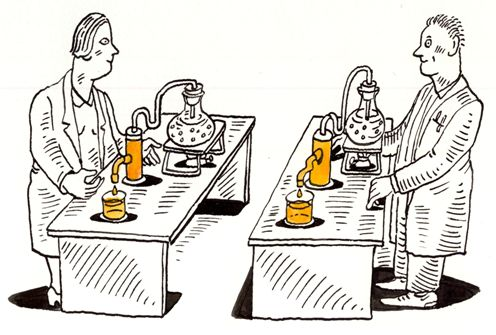
\includegraphics[width=\textwidth,keepaspectratio]{../resources/reproducibility.jpg}
            \end{figure}
        \end{column}
    \end{columns}
\end{frame}

\begin{frame}
    \begin{columns}
        \begin{column}{0.5\textwidth}
            Is reproducibility really that important?
        \end{column}
        \begin{column}{0.5\textwidth}
            \begin{figure}
                \centering
                
\includegraphics[width=\textwidth,keepaspectratio]{../resources/signature.jpg}
            \end{figure}
        \end{column}
    \end{columns}
\end{frame}

\begin{frame}
    \centering It depends
\end{frame}

\begin{frame}
    Threat modeling some upstream software sources:
    \begin{itemize}
        \item Malicious changes to source code
        \item User/System compromise within the development chain
        \item Watering-hole attacks
        \item Any more?
    \end{itemize}
\end{frame}

\begin{frame}
    Reproducibility protects us from 2 of 3 of these
    \begin{itemize}
        \item \st{Malicious changes to source code}
        \item User/System compromise within the development chain
        \item Watering-hole attacks
    \end{itemize}
\end{frame}

\begin{frame}
    \centering
    How does Nix provide reproducibility?
\end{frame}

\begin{frame}
    \centering
    We'll consider a simple binary on most Linux systems: find
\end{frame}

\begin{frame}
    \centering
    /nix/store\textbf{/jjvw20r6pz3ff7pn91yhvfx8s7izsqan}-findutils-4.8.0/bin/find
\end{frame}

\begin{frame}
    
\includegraphics[width=\textwidth,keepaspectratio]{../resources/what-in.jpg}
\end{frame}

\begin{frame}
    \centering Anyone know what this would look like on Ubuntu?
\end{frame}

\begin{frame}
    \begin{columns}
        \begin{column}{0.5\textwidth}
            \centering
            Ubuntu:
            \begin{figure}
                \centering
                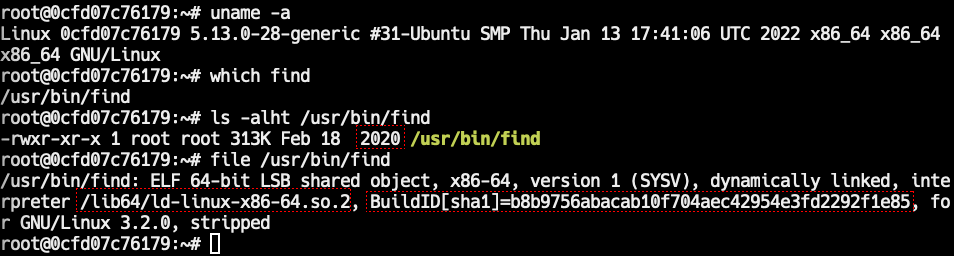
\includegraphics[width=\textwidth,keepaspectratio]{../resources/ubuntu-find.png}
            \end{figure}
        \end{column}
        \begin{column}{0.5\textwidth}
            \centering
            Nix:
            \begin{figure}
                \centering
                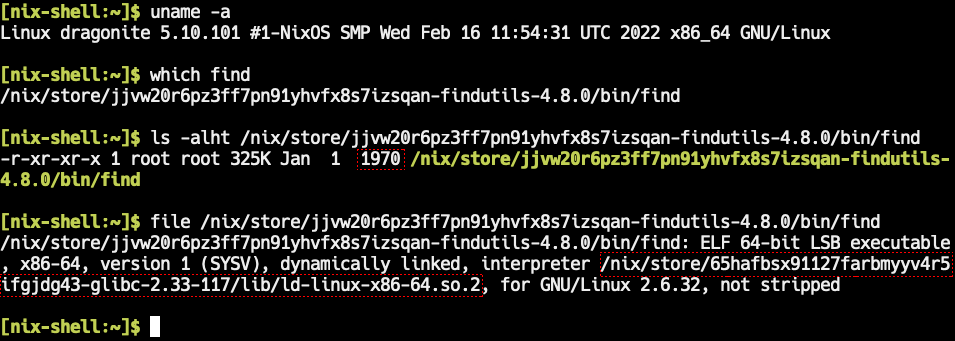
\includegraphics[width=\textwidth,keepaspectratio]{../resources/nix-find.png}
            \end{figure}
        \end{column}
    \end{columns}
\end{frame}

\begin{frame}
    There's a few things to note in these images, taking for example Ubuntu:
    \begin{figure}
        \centering
        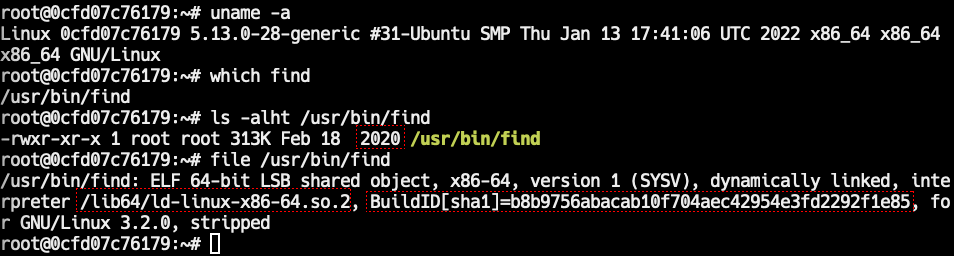
\includegraphics[width=\textwidth,keepaspectratio]{../resources/ubuntu-find.png}
    \end{figure}
\end{frame}

\begin{frame}
    \begin{figure}
        \centering
        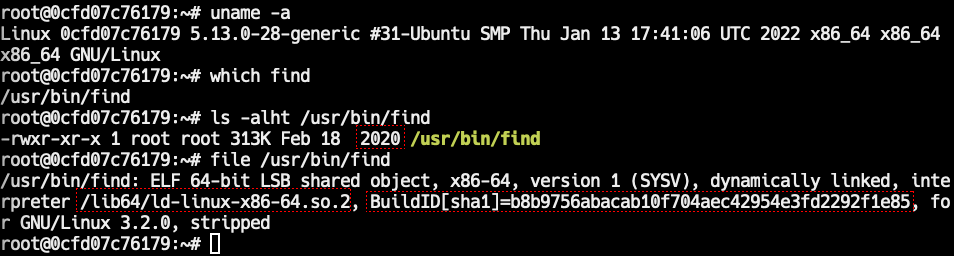
\includegraphics[width=\textwidth,keepaspectratio]{../resources/ubuntu-find.png}
    \end{figure}
    \begin{itemize}
        \item File metadata regarding the create time has been left in
        \item The linker is a pretty standard location for this
        \item We've got a build ID that links to Canonical's build
    \end{itemize}
\end{frame}

\begin{frame}
    \centering
    Do we trust this binary?
\end{frame}

\begin{frame}
    \centering
    I mean, generally yeah we probably could.
\end{frame}

\begin{frame}
    \centering
    Could we reproduce the \textit{exact same binary} given the source code of \textbf{\textit{find}}?
\end{frame}

\begin{frame}
    \centering
    
\includegraphics[width=\textheight,keepaspectratio]{../resources/rabbit-hole.jpg}
\end{frame}

\begin{frame}
    We could probably, but we'd need to:
    \begin{itemize}
        \item Utilise a build system that applies the same build process as the original
        \item Ensure we had no volatile inputs (network data is consistent and trustworthy \& more)
        \item Utilise the same makefile (was it the \href{https://git.savannah.gnu.org/cgit/findutils.git/tree/Makefile.am}{\color{blue}original GNU} one or a modified one?)
        \item Ensure the compiler zeros all memory before value initialisation
        \item Uses the same version information
        \item Ensure the compiled output has the same timestamp
        \item Ensure no locale-specific options have side effects on the compile
        \item Ensure stable ordering for outputs (Do python dictionaries always yield their keys in the same order?)
        \item Eliminate PRNG in compile if relevant
        \item Ensure debug symbols are removed (may contain environment values specific to us)
    \end{itemize}
\end{frame}

\begin{frame}
    \centering
    Was that last slide cutoff?
\end{frame}

\begin{frame}
    \centering
    Yep! Those considerations are just the tip of the iceberg!
    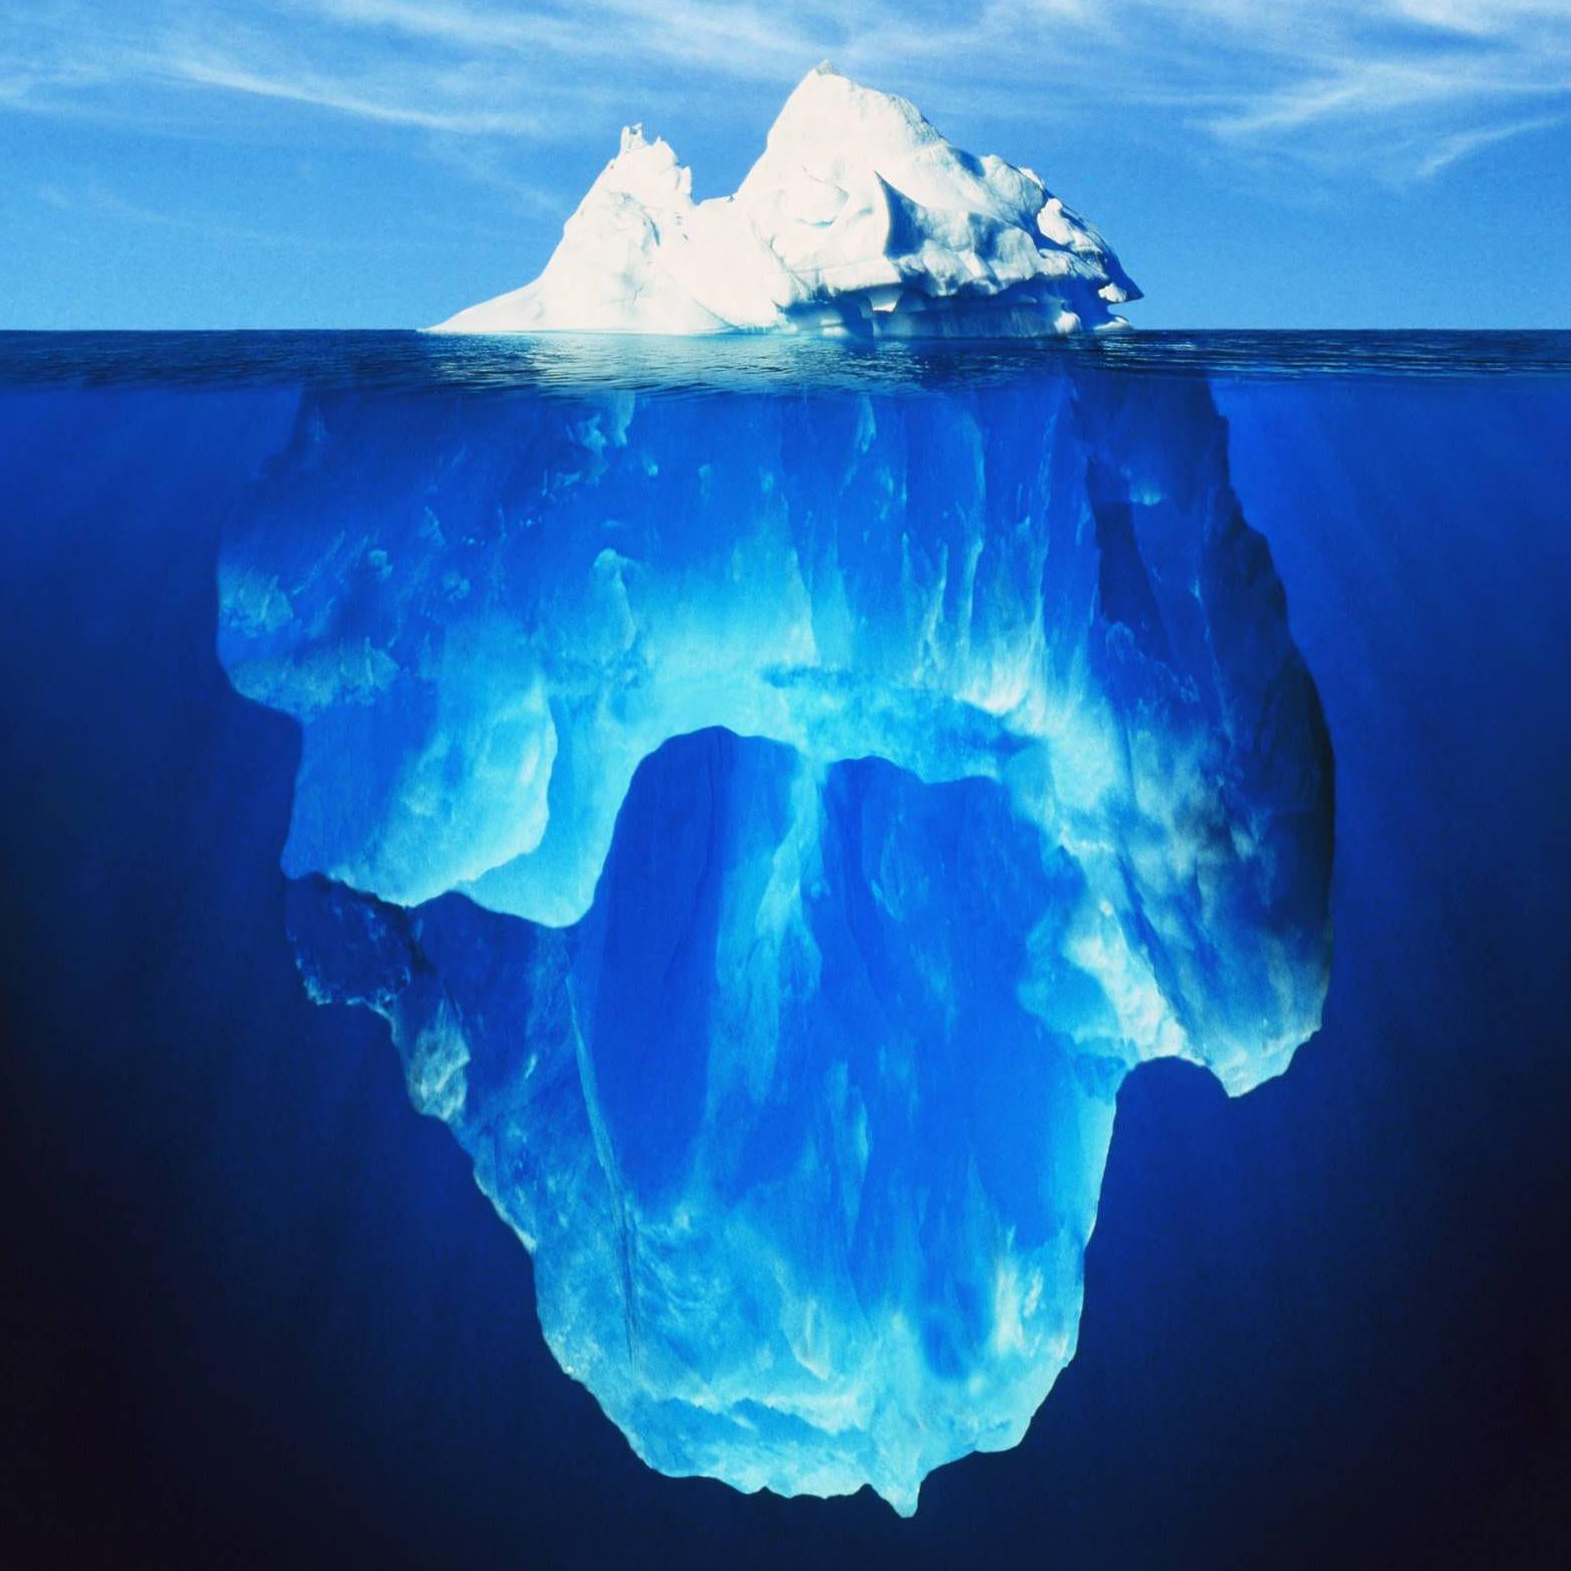
\includegraphics[width=\textwidth]{../resources/iceberg.png}
\end{frame}

\begin{frame}
    \centering
    So how does Nix avoid all of these pitfalls?
\end{frame}

\begin{frame}
    \centering
    Nix creates \textit{derivations} which is just a fancy word for builds.
    \par\vspace{5mm}
    Derivations are however distinct to not only the software version you're building.
    But all of the inputs also
\end{frame}

\begin{frame}
    \centering
    Because of this feature, we can \textit{know} that the method in which we build and install our
    software of choice is \ul{the same} as what the author of the derivation intended.
\end{frame}

\begin{frame}
    \centering
    Why is it provable with Nix?
\end{frame}

\begin{frame}
    \centering
    In short: the generated path is linked to both the software as well as all inputs
    within the dependency tree
    \par\vspace{5mm}
    /nix/store\textbf{/jjvw20r6pz3ff7pn91yhvfx8s7izsqan}-findutils-4.8.0/bin/find
\end{frame}

\begin{frame}
    Steps to generate this hash (paraphrasing):
    \begin{itemize}
        \item SHA256 the descriptor of a build
        \item Recursively SHA256 files required in the build process in a deterministic order, truncating output then base32
        \item ???
        \item ???
        \item Profit!
    \end{itemize}
\end{frame}

\begin{frame}
    \centering
    Are all Nix configs and packages reproducible?
\end{frame}

\begin{frame}
    \centering
    Questions on any of this?
    
\includegraphics{../resources/question-2.png}
\end{frame}

\subsection{Reliability}

\begin{frame}
    \centering
    Reliability
\end{frame}

\begin{frame}
    \centering
    
\includegraphics[width=\textheight,keepaspectratio]{../resources/linux-wont-boot.png}
\end{frame}

\begin{frame}
    \centering
    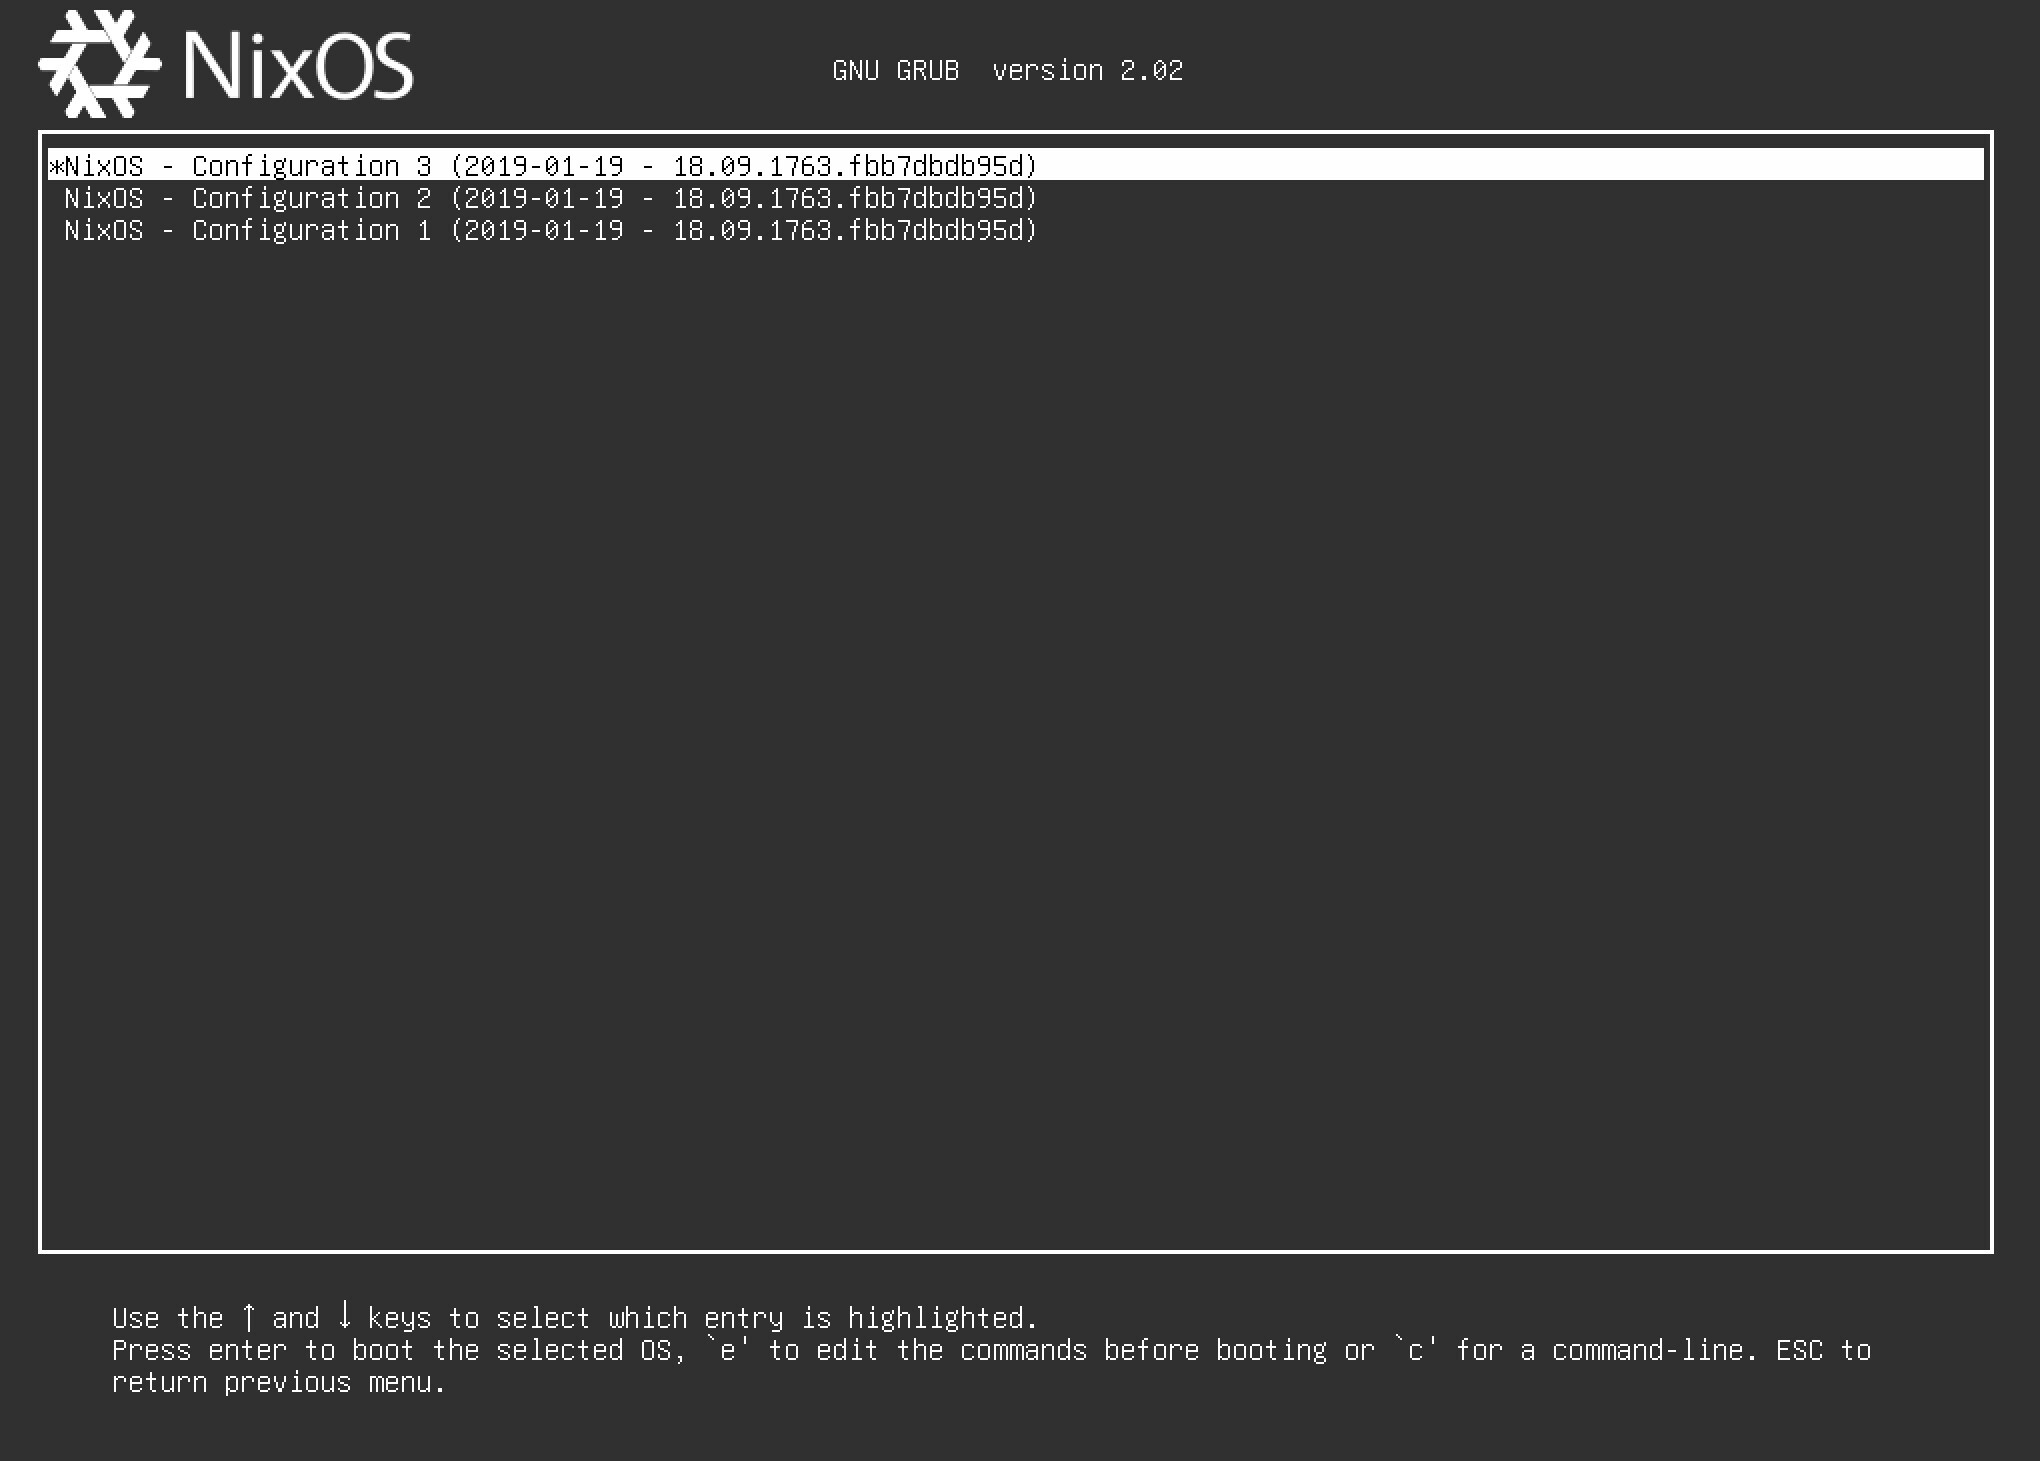
\includegraphics[width=\textheight,keepaspectratio]{../resources/nix-grub-bios.jpg}
\end{frame}

\begin{frame}
    \centering
    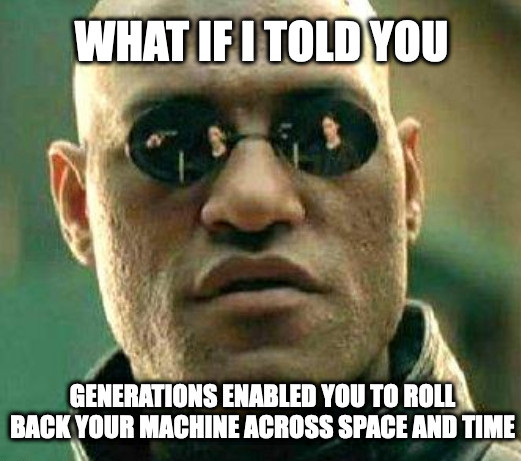
\includegraphics[width=\textheight,keepaspectratio]{../resources/what-if-i-told-you.jpg}
\end{frame}

\begin{frame}
    Downsides of generations?
    \begin{itemize}
        \item Well, mostly just disk space
    \end{itemize}
    But who doesn't have the ability to utilise multi-gigabyte drives nowadays?
\end{frame}

\begin{frame}
    \centering
    Resolving disk space issue?
    \par\vspace{5mm}
    Easy! Nix has a garbage collector!
    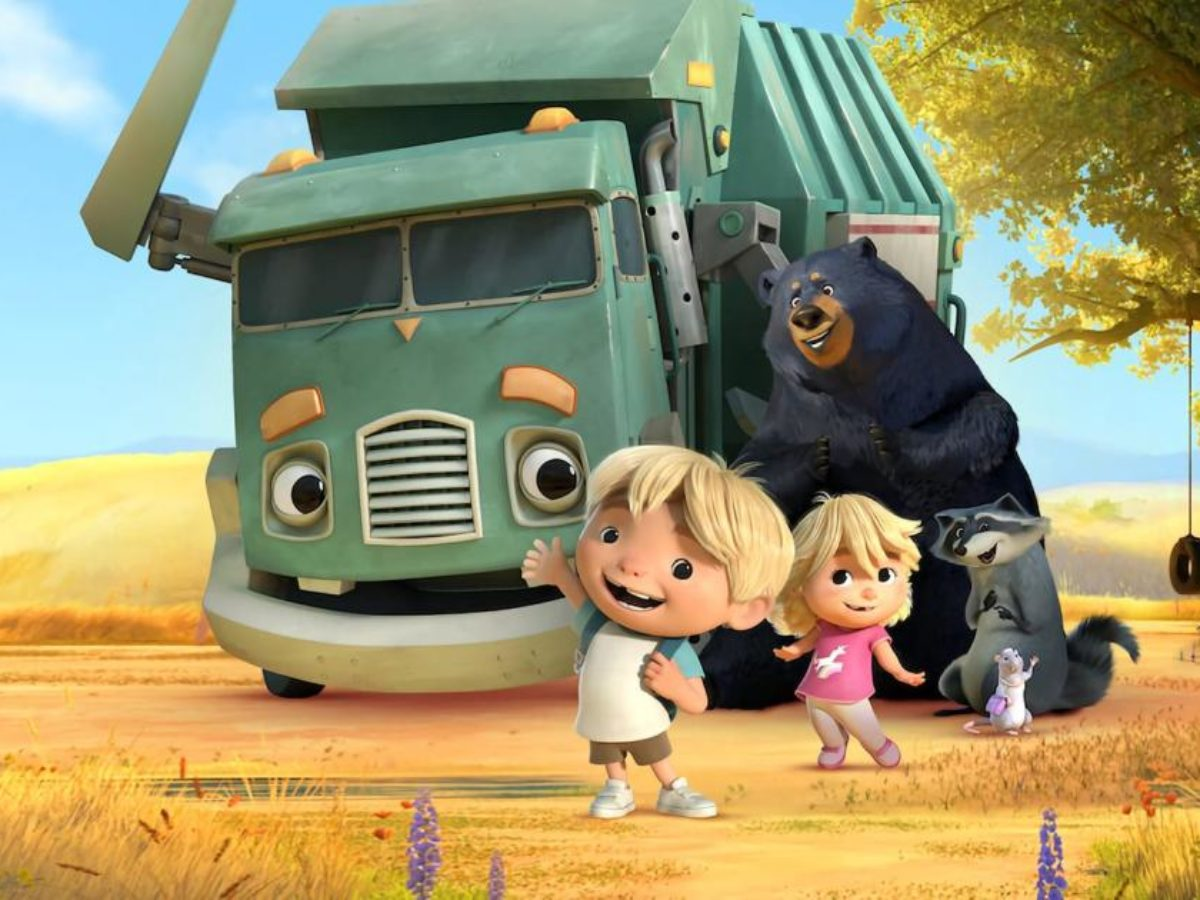
\includegraphics[width=\textheight,keepaspectratio]{../resources/trash-truck.jpg}
\end{frame}

\begin{frame}
    \centering
    Where to from here?
\end{frame}

\begin{frame}
    \centering
    Fin!
\end{frame}

\end{document}